\chapter{Conceptos Financieros }
\section{Acciones,Opciones, Calls y Puts}
Una \textbf{acción} es un título emitido por una sociedad que representa el valor de las fracciones iguales en que se divide su capital social. Que además la empresa puede decidir ponerlas en venta a los inversores, en el cual tiene clasificaciones:
	\begin{itemize}
		\item Acciones de clase A 
		\item Acciones de clase B
	 
	\end{itemize}
 	
 		\textbf{ Acciones de clase A }: Son aquellas acciones en las cuales, uno puede ejercer dividendos\footnote{Es la parte del beneficio de una empresa que se reparte entre los accionistas de una sociedad.} y toma de decisiones de la empresa.
 		\newline
 		\textbf{ Acciones de clase B}: Son aquellas que no ejercen derechos de la empresa ni cobrar dividendos, solo son acciones con cierto valor, por lo general están cotizadas en una \textbf{bolsa de valores}\footnote{Es una organización privada que brinda las facilidades necesarias para que sus miembros, atendiendo los mandatos de sus clientes, como realizar venta y compra de valores, tales como bonos, acciones de sociedades.}.
 		\newline
 		Para las acciones de clase B las empresas utilizan esas inversiones para proyectos, ampliaciones, o cosas que necesiten la empresa; pero las empresas están obligadas a dar sus estados financieros, eso quiere decir que están obligados a presentar su contabilidad y sus ventas.  \newline
	Con la siguiente gráfica podemos apreciar como se comporta una acción de clase B, esta gráfica fue sacada de Yahoo finance en donde esta abierta para todo publico para cotizar acciones.
\begin{figure}[h]
	\centering
	\label{Accion de Google cotizadas en NASDAQ}
	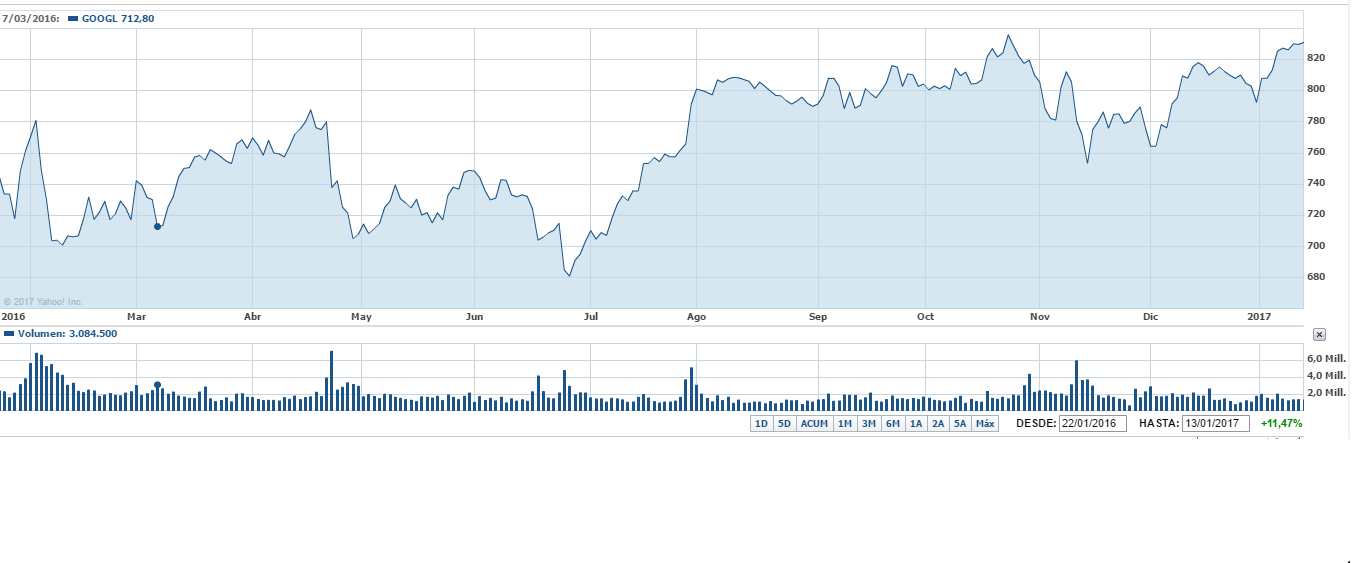
\includegraphics[width=1.2\linewidth]{google}\\
	\caption[Titulo en el índice de figuras (opcional)]{Acción de Google  cotizada en la bolsa de valores de U.S.A}
\end{figure}
		\newpage
		Como se puede apreciar en la gráfica ( él lado derecho) es el valor del precio de una acción en dolares, en la parte inferior tenemos el \textbf{volumen}\footnote{El volumen de una acción es el numero de transacciones. } de la acción.
		 \newline
		 las acciones se comportan de forma estocástica, dado que tienen un cierre y una apertura, por lo general una acción vista en forma diaria se aprecia como en la gráfica 1.
		  \newline
		 \begin{figure}[h!]
		 	\centering
		 	\label{Apertura y cierre}
		 	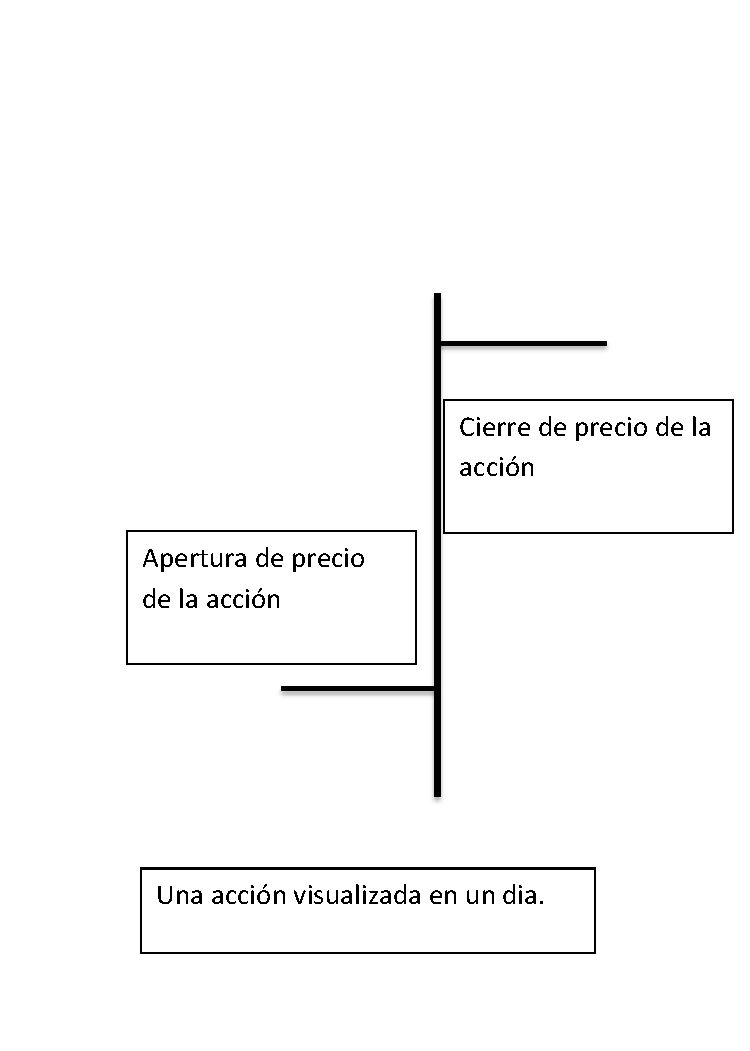
\includegraphics[width=0.35\linewidth]{a}\\
		 	\caption[Titulo en el índice de figuras (opcional)]{Comportamiento de una acción cuando el mercado esta abierto.}
		 \end{figure}
		  \newpage
Una \textbf{opción} es un contrato que se da a su comprador el derecho pero no la obligación a comprar o vender bienes, hasta una fecha concreta existen dos tipos de opciones:
	\begin{itemize}
		\item Opción de compra (Calls) 
		\item Opción de venta (Puts) 
	
	\end{itemize}

Un \textbf{call} es una opción de compra, en el que uno tiene el derecho pero no la obligación de comprar las acciones asociadas; si se emite un \textbf{Call} tiene la obligación de entregar las acciones asociadas al precio de ejecución.    	
		\newline
Un \textbf{Put} es una opción de venta, en el que uno tiene el derecho pero no la obligación de vender las acciones asociadas; si se emite un \textbf{Put} tiene la obligación de entregar las acciones asociadas al precio de ejecución.    	
\newline		
\begin{defn}Un \textbf{ Call} es $ C=Max(0,S-X) $;donde $ X $ es el precio de la opción y $ S $ es el precio de la acción.	
	\end{defn}
\begin{defn}Un \textbf{ Put} es $ C=Max(0,X-S) $;donde $ X $ es el precio de la opción y $ S $ es el precio de la acción.	
\end{defn}	
\subsection{Rentabilidad a lo largo}
Una rentabilidad a lo largo para un \textbf{call} es cuando la acción sube de precio entonces, el precio de la opción sube.	
\newline 
Aquí va una imagen
\newline 
Una rentabilidad a lo largo para un \textbf{put} es cuando la acción baja de precio entonces, el precio de la opcion sube.	
\newline 
Aquí va una imagen
\newline 
\subsection{Rentabilidad a lo corto}
Una rentabilidad a lo largo para un \textbf{call} es cuando la accion baja de precio entonces, el precio de la opcion naja.	
\newline 
Aqui va una imagen
\newline 
Una rentabilidad a lo corto para un \textbf{put} es cuando la accion sube de precio entonces, el precio de la opcion baja.	
\newline 
Aqui va una imagen
\section{Valor Intriseco}
Es cuando el valor del bien menos el derecho que vale, sus tres formas que se pueden dar son:
	\begin{itemize}
		\item In the Money
		\item At the Money 
		\item out of the Money
	
	\end{itemize}

Si es \textbf{In the Money} para un \textbf{call} es si el precio de ejecución de un call es mayor que el precio de la acción en pocas palabras $ S > X $.
\newline
Si es \textbf{In the Money} para un \textbf{put} es si el precio de ejecución de un put es menor que el precio de la accion en pocas palabras $ X > S $.
\newline
Si es \textbf{At the Money} para un \textbf{Call} es si el precio de ejecución de un call es igual que el precio de la accion en pocas palabras $ S = X $.
\newline
Si es \textbf{At the Money} para un \textbf{Put} es si el precio de ejecución de un put es igual que el precio de la accion en pocas palabras $ S = X $.
\newline
Si es \textbf{out the Money} para un \textbf{Call} es si el precio de ejecución de un call es menor que el precio de la accion en pocas palabras $ S < X $.
\newline
Si es \textbf{out the Money} para un \textbf{Put} es si el precio de ejecución de un put es mayor que el precio de la acción en pocas palabras $ X < S $.

\begin{defn}Una \textbf{ Prima de una opción} es el precio del contrato o de la opción en pocas palabras es: 
	\begin{equation}\label{eq1}
	Prima= V.I +V.T
	\end{equation}
	Donde $ V.I $ es el valor intrínseco y $ V.T $ es el valor del tiempo.
\newline
El \textbf{Valor del tiempo} de una opción se desvanece con mayor rapidez a partir de sus últimos días de expiran.
\section{Estrategias sobre opciones}
Las estrategias sobre opciones implican tomar posiciones en opciones, los activos subyacentes, y los prestamos otorgados, las 4 posiciones que tienen son: \textbf{call a lo largo, call a lo corto, put a lo largo y un put a lo corto}. Las estrategias pueden ser de tres tipos:
		\begin{itemize}
			\item Alcista
			\item Mercado pesimista 
			\item Neutral
			
		\end{itemize}
En términos de perspectivas del mercado pueden ser tres:\textbf{Agresivo, defensivo y Riesgos } el termino de riesgo viene por obtener beneficios en mercados calmados.		
	
			\section{Valor del dinero en el tiempo}
			El \textbf{interés} es el costo de pedir prestado dinero, entonces sea $ r $ el interés anual, si el interés es compuesto una vez por año , entonces el valor del futuro ($ VF $)	de una cantidad inicial  $ P $ después de n años es.
			\begin{equation}\label{eq0}
		    VF=P(1+r)^{n}
			\end{equation}
			el valor presente ($ VP $) que es el valor del día de hoy se puede escribir como:		
							\begin{equation}\label{eq0}
							P=VF(1+r)^{-n}
							\end{equation}
				\subsection	{Valor presente}
				Sea ($ VP $) y sea $ C_{n} $ un fluido de dinero a través del tiempo $ 1,2,\cdots,n $ y $ r $ el interés anual es:
						\begin{equation}\label{eq0}
						VP= \dfrac{C_{1}}{(1+r)}+\dfrac{C_{2}}{(1+r)^{2}}+\cdots+\dfrac{C_{n}}{(1+r)^{n}}
						\end{equation}	
				\section{Opciones arbitrarias}		
						Una oportunidad de arbitraje sin riesgo es aquella que, sin ninguna inversión inicial, genera una rentabilidad no negativa en todas las circunstancias y rendimientos positivos. En un mercado eficiente.
						\textbf{El principio dominante del portafolio} dice que él portafolio A debería ser mas valioso que el portafolio B si la rentabilidad de A es al menos tan buena bajo todas las circunstancia.\newline
						Derivando las relaciones libres de arbitraje que los valores de las opciones deben de satisfacer. Estas relaciones son independientes del modelo probabilístico del precio de acciones, solo asumimos que no hay costo de transacción y los prestamos están disponibles a la tasa de interés sin riesgo, las tasas de interés son no negativas y no hay oportunidad de arbitraje, simplificando esto tenemos que el tiempo sea cero. $ VP(x) $ donde $ x $ son los dolares a expirar. 
							\begin{equation}\label{eq0}
							VP(x)= xd(\tau) 
							\end{equation}
							
							Donde $ \tau $ es el tiempo a expirar
							\begin{lem}\label{lmcp11}
								En la bolsa americana un $ call $ y un $ put  $ con tiempo mas largo a la expiración no puede valer menos que un $ call $ y un $ put $ en un menor tiempo de expiración 
							\end{lem}
							
							\begin{lem}\label{lmcp11}
							La opción $ Call $ y $ put $ con un precio de ejercicio mas alto (mas bajo) respectivamente no puede valer mas que un $ call $ y un $ put $ idéntico con un precio de ejercicio mas bajo  (más alto).
							\end{lem}
							
							\begin{lem}\label{lmcp11}
							La diferencia en los valores de dos opciones por lo demás idénticas no puede ser mayor que la diferencia de sus precios de ejercicio
							\end{lem}
							
								\begin{proof} 
									Consideremos los Calls nada mas. Sea 2 precios de ejercicio tal que $ X_{1}<X_{2} $. Asumamos que $ C_{1} - C_{2}<X_{2}-X_{1} $ en lugar. Compramos el precio mas bajo $ C_{2} $ y escribimos a $ C_{1} $ el precio mas alto, generando retornos positivos y depositando $ X_{2}-X_{1} $ en una cuenta sin riesgo en un banco.
									  \newline
									  Supongamos que se ejecuta $ C_{1} $ antes del tiempo de expiracion, tendríamos dos casos. Si $ C_{2} >S-X_{1}$, entonces vendemos $ C_{2} $, la rentabilidad de la venta seria $ C_{2}-(S-X_{1})>0 $ de lo contrario $ C_{2} $ realizaría un flujo de caja de $ X_{1}-X_{2} < 0  $ , en ambos casos cerramos la transacción con el dinero en el banco realizaríamos un flujo de efectivo no negativo. \newline
									  Supongamos ahora que no se ejecuta antes de la fecha de vencimiento $ C_{1} $, entonces el flujo de efectivo es 0, $ X_{1}<S $ , y $ X_{1}-X_{2} < 0 $, respectivamente si $ S \leq X_{1} $, $ X_{1}<S<X_{2} $ y $ S\leq X_{2} $, el flujo sigue siendo no negativo despues de que el dinero se agrega en la cuenta bancaria. 
									   
								\end{proof}
								\subsection	{La paridad de una opción }
							Supongamos que la acción no paga dividendos en efectivo o que las opciones están protegidas para que los valores de las opciones sean insensibles a los dividendos en efectivo. Por lo tanto, los resultados de las opciones protegidas no se enumeran por separado.	\newline
							El principio del no arbitraje implica que la inversión inicial establece que el portafolio también debe de ser nula. Con esto tenemos la paridad para las opciones europeas:
							
							\begin{equation}\label{eq0}
							C=P+S-VP(x)
							\end{equation}
							Consideremos $ C-P= S-VP(x) $ lo que implica que un $ call  $ a lo largo y un $ put $ a lo corto ponen a una posición larga en acciones y toman prestado $ VP $ del precio de ejercicio en pocas palabras es tomar una acción a lo largo como comprar acciones en margen. entonces la paridad del call y del put seria:
								\begin{equation}\label{eq0}
								C=(S-X) + [X-VP(x)]+P \geq S-X
								\end{equation}
								Por que $ C\geq 0 $ dado que $ C\geq max (S-X) $, el valor intrínseco; un call americano no puede valer menos que su valor intrínseco. por lo tanto tenemos los siguientes lemas. 
								\begin{lem}\label{lmcp11}
									Un call de una acción que no paga dividendos nunca vale menos que su valor intrínseco 
									
								\end{lem}
									\begin{lem}\label{lmcp11}
									Para los put europeos, $ P\geq max(VP(X)-S,0) $ 	
									\end{lem}
									\begin{thm}
									Un Call americano se ejercerá solo al momento del vencimiento o justo antes de que se venza los dividendos
									
									\end{thm}
									\subsection	{Convexidad de los precios de la opciones }
										\begin{thm}
										 la convexidad de los precios de las opciones, tenemos que para tres calls con precio de ejercicio idénticos $ X_{1}<X_{2}<X_{3} $, tenemos el: 
											\newline
											$ C _{X_{2}} \leq \lambda C _{X_{1}} + (1-\lambda) C _{X_{3}} $ , $ P _{X_{2}} \leq \lambda P _{X_{1}} + (1-\lambda) P_{ X_{3}} $
											\newline
											Donde $ \lambda = (X_{3}-X_{2}/(X_{3}-X_{1})) $	
										\end{thm}
									\begin{proof} 
									Supongamos que no es convexa, primero anotamos en nuestro portafolio a $  C _{X_{2}}  $ entonces compramos $  \lambda C _{X_{1}}  $, y compramos $ (1- \lambda) C _{X_{3}}  $, estamos generando un flujo  efectivo positivo. si call a lo corto no es ejecutado antes del día de expiracion manteniendo los calls hasta la expiracion el flujo de caja es descrito como:\newpage
								
								
							\begin{longtable}{|l|l|l|l|l|}
									\hline 
									& $ S\leq X_{1} $ & $ X_{1}< S \leq X_{2} $  & $ X_{2}<S<X_{3} $  & $ X_{3}\leq S $  \\ 
									\hline 
									Call descrito en $ X_{2} $& 0  & 0  & $ X_{2}-S $ & $ X_{2}-S $  \\ 
									\hline 
									$ \lambda $ calls compradas en $ X_{1} $& 0  & $ \lambda (S-X_{1}) $ &$ \lambda (S-X_{1}) $  & $ \lambda (S-X_{1}) $  \\ 
									\hline 
									$1- \lambda $ calls compradas en $ X_{3} $& 0  & 0  & 0 & $(1- \lambda )(S-X_{3}) $   \\ 
									\hline 
									& 0 &$ \lambda (S-X_{1}) $  & $ \lambda (S-X_{1}) $ + ($ X_{2}-S $ )  & 0 \\ 
									\hline 
							\end{longtable}  
								 Tenemos que el flujo de dinero es 0 o positivo, esto es una propiedad de arbitraje.
								 \newline
								 Supongamos que el call a lo corto se ejerce anticipadamente cuando el precio de la acción $ S $. Si 	$  \lambda C _{X_{1}} + (1-\lambda) C _{X_{3}}> S-X_{2} $, vendemos calls a lo largo para generar un flujo de dinero de 	$  \lambda C _{X_{1}} + (1-\lambda) C _{X_{3}} - (S-X_{2})>0 $. De lo contrario, ejecute calls a lo largo y entregue las acciones, entonces el flujo neto de  dinero es $ -\lambda X_{1}- (1-\lambda)X_{3}+X_{2} = 0  $De nuevo tenemos que es una propiedad arbitraria. \newline
								 Por el lema 2.3, sabemos que la pendiente del valor de un call (put), cuando se traza con el precio de ejercicio, es a lo mas uno (menos uno, respectivamente). esto prueba que se forma la convexidad.
									 \end{proof}
									 
									 \section	{Conceptos de los modelos financieros }
									En esta parte solo sera una breve definición, y en el otro capítulo sera el contenido mas detallado.
									\subsection	{Árbol binomial}
									
									En el  modelo del Árbol binomial en opciones y en acciones, tenemos que el tiempo es discreto y una medida en periodos, el modelo asume que si el precio actual de la acción es$ S $, puede subir su precio $ Su $ con una probabilidad $ q $, ahora si el precio de la acción baja $ Sd $ tiene que tener una probabilidad de $ 1-q $, donde $ 0<q<1 $ y $ d<u $. En efecto, $ d<R<u $ donde $ R=e^{\widehat{r}} $ con $ \widehat{r} >0 $ , Resultando que se necesita 6 datos conocidos para determinar el valor de la opción basándose en las condiciones de arbitraje: $ S $, $ u $,$ d $,$ X $,$ \widehat{r} $ y el numero de periodo antes de la expiración.
									\newline
									Aqui va una imagen
									\subsection	{Simulación Monte Carlo}
									La simulación de Monte Carlo es una técnica que utiliza muestreo aleatorio para estimar los resultados del modelo. Las estadísticas calculadas sobre estos resultados, tales como media, desviación estándar y percentiles. Entonces el método de Monte Carlo se puede interpretar como el valor esperado de una variable aleatoria $ Z $ definida como  
										\begin{equation}\label{eq0}
										Z=\dfrac{max (0,Su^{j}d^{n-j} - X)}{R^{n}}
										\end{equation}
										Con probabilidad $ b (j;n,p) $ con $ 0\leq j\leq n	  $
										
											\subsection	{Black- Scholes}
											Es la formula matemática utilizada para obtener los precios de las opciones sobre divisas fijas, fecha caducidad, el modelo genera precios basado e un conjunto de ideales relacionados con la volatilidad, distribución normal y las densidades de probabilidad, los principales impulsadores del modelo de fijación de precios son el precio de divisas, valor intrínseco, el tiempo de caducidad y la volatilidad, el la formula de Black- Scholes esta dado como: 
												\begin{equation}\label{eq0}
												C=S N(x) - Xe^{-r\tau}N(x-\sigma\sqrt{\tau})
												\end{equation}
												y para Put
													\begin{equation}\label{eq0}
													P=Xe^{-r\tau} N(-x+\sigma\sqrt{\tau}) - SN(-x)
													\end{equation}
													Donde $ x=\dfrac{Ln(S/X)+(r+\frac{\sigma^{2}}{2})}{\sigma \sqrt{\tau}} $
													
													